
% np.array([]), np.arange(), np.zeros(),
% np.loadtxt("file", dtype=object, delimiter='!!!')
% +, -, *, /
% np.sqrt()
% np.round( , num_decimals)
% np query syntax

% indexing, slices

\chapter{Arrays in Python (1 of 2)}

\index{array!in NumPy}
\index{ndarray@\texttt{ndarray} (NumPy)}
\index{list@\texttt{list}, plain-ol'}
There are several candidates in the Python language for representing the type
of array structure we introduced in chapter~\ref{ch:aggregateData}. One is the
plain-ol' Python \textbf{\texttt{list}}, which you may have used if you've
taken a computer science course in Python. Turns out, \texttt{list}s are going
to be too slow for us once we start dealing with a lot of data, plus there are
a lot of things that it won't do for us automatically that are handy to have.
Another choice is the Pandas \texttt{Series} which we'll actually cover in
chapter~\ref{ch:pythonAssocArrays} -- oddly, that one turns out to do too
\textit{much}, rather than too little, for our purposes here. A happy medium is
the \textbf{\texttt{ndarray}} from the NumPy package\footnote{Most people seem
to pronounce this ``NUM-pie,'' although I've heard ``NUM-pee'' as well. Pick
your poison.}. Before we do that, however, we need to learn what a ``package''
actually is, and how to use one.

\section{Packages}
\index{package}

Back in my day (circa 1990's) when someone wanted to write a computer program,
they wrote the entire thing themselves, line by line. Everything you needed to
do -- from something complex like making a remote network connection to
something simple like computing the average of some numbers -- was up to you to
build. Code sharing over the Internet just wasn't much of a thing.

Today, the reverse is true. When you write a complex data analysis program,
\textit{most} of the code will actually be written by others, if you do it
right. This is because many, many smart people across the globe have written
snippets of code to do all the common (and some not-so-common) things you'll
want to do, and your job is to string them all together. Put another way:
you're given most of the Legos\textsuperscript{\textregistered} -- and even a
bunch of pre-assembled chunks made with dozens of
Legos\textsuperscript{\textregistered} each -- and your job is to construct
your masterpiece out of those building blocks.

\index{package}
\index{importing (a package)}
\index{package}
\index{calling a function@``calling'' a function}
\index{calling a method@``calling'' a method (on a variable)}
In Python, a \textbf{package} is a repository of useful functions and methods
that someone else has written. By \textbf{import}ing a package into your
program, you're making all those useful things available to you. Your own code
can then call those functions/methods whenever you see fit. It's the modular,
organized, and elegant way to do things, in addition to saving a ton of time.

The first package we'll use is called \textbf{NumPy}, which stands for
``Numerical Python.'' To import it, you should include this exact line of code
in the \textit{first} Code cell of your Notebook:

\begin{Verbatim}[fontsize=\small,samepage=true,frame=single,framesep=3mm]
import numpy as np
\end{Verbatim}

Note that it's in all lower-case letters. Once that cell has been executed, you
now have access to all the NumPy ``stuff,'' which is the subject of this
chapter.

\section{The NumPy \texttt{ndarray}}
\label{sec:creatingArrays}

\index{array}
\index{ndarray@\texttt{ndarray} (NumPy)}
\index{matrix}
The actual data type that the NumPy package provides is called an
\texttt{ndarray}, which stands for ``n-dimensional array.'' If that sounds
heady, it kind of is, although in this course we're only ever going to use a
\textit{one}-dimensional array, which is super simple to understand. In fact,
it looks exactly like the examples in Figure~\ref{fig:array}
(p.~\pageref{fig:array}). ``One-dimensional'' just means that there is a single
index number, and the elements are all in a line.\footnote{A two-dimensional
array is a spreadsheety-looking thing also called a \textbf{matrix}. Each
element has \textit{two} index numbers: a row and a column. A three-dimensional
array is a cube, with three index numbers needed to specify an element.
\textit{Etc.}}

\subsection{Creating \texttt{ndarray}s}

There are many different ways to create an \texttt{ndarray}. We'll learn four
of them.

\subsubsection{Way 1: \texttt{np.array([])}}

\index{array@\texttt{array()} function (NumPy)}
The first is to use the \texttt{array()} function of the NumPy package, and
give it all the values explicitly. Here's the code to reproduce the
Figure~\ref{fig:array} examples:

\begin{Verbatim}[fontsize=\scriptsize,samepage=true,frame=single,framesep=3mm]
followees = np.array(['@katyperry','@rihanna','@Cristiano','@TheEllenShow'])
balances = np.array([1526.73, 98774.91, 1000000, 4963.12, 123.19])
\end{Verbatim}

\index{boxies (square brackets)}
\index{[]@\texttt{[]} (boxies)}
\index{bananas (parentheses)}
\index{()@\texttt{()} (bananas)}
It's simple, but don't miss the syntactical gotcha: \textit{you must include a
pair of boxies inside the bananas.} Why? Reasons.\footnote{For the experienced
reader, what we're actually doing here is creating a plain-ol' Python list
(with the boxies), and then calling the \texttt{array()} function with that
list as an argument.} For now, just memorize that for this function -- and this
function only -- we use ``\texttt{([}\textsl{...stuff...}\texttt{])}'' instead
of ``\texttt{(}\textsl{...stuff...}\texttt{)}'' when we call it.

\index{package}
\index{function}
\index{method}
By the way, the attentive reader might object to me calling \texttt{array()} a
function, instead of a method. Isn't there a word-and-a-dot before it, and
isn't that a ``method thing?'' Shrewd of you to think that, but actually no,
and the reason is that ``\texttt{np}'' isn't the name of a variable, but the
name of a \textit{package}. When we say ``\texttt{np.array()}'' what we're
saying is: ``Python, please call the \texttt{array()} function \textit{from the
\texttt{np} package}.'' The word-and-dot syntax does double-duty.

\index{type@\texttt{type()}}
We can call the \texttt{type()} function, as we did back on
p.~\pageref{typeFunction}, to verify that yes indeed we have created
\texttt{ndarray}s:

\begin{Verbatim}[fontsize=\small,samepage=true,frame=single,framesep=3mm]
print(type(followees))
print(type(balances))
\end{Verbatim}

\begin{Verbatim}[fontsize=\small,samepage=true,frame=leftline,framesep=5mm,framerule=1mm]
numpy.ndarray
numpy.ndarray
\end{Verbatim}

\index{dtype@\texttt{.dtype} (NumPy)}
This is useful, but sometimes we want to know what underlying atomic data type
the array is comprised of. To do that, we attach ``\texttt{.dtype}''
(confusingly, \textit{without} bananas this time) to the end of the variable
name. ``\texttt{.dtype}'' stands for ``data type.'' Here goes:

\begin{Verbatim}[fontsize=\small,samepage=true,frame=single,framesep=3mm]
print(type(followees))
print(type(balances))
\end{Verbatim}

\begin{Verbatim}[fontsize=\small,samepage=true,frame=leftline,framesep=5mm,framerule=1mm]
dtype('<U13')
dtype('float64')
\end{Verbatim}

\index{bit@bit (``binary digit'')}
Whoa, what does \textit{that} stuff mean? It's a bit hard on the eyes, but let
me explain. The underlying data type of \texttt{followees} is (bizarrely)
``\texttt{<U13}'' which in English means ``strings of Unicode
characters\footnote{A ``Unicode character'' is just a fancy way of saying ``a
character, which might not be English.'' NumPy is capable of storing more than
just a-b-c's in its strings; it can store symbols from Greek, Arabic, Chinese,
\textit{etc.} as well.}, each of which is 13 characters long or less.'' (If you
bother to count, you'll discover that the longest string in our
\texttt{followees} array is the last one, \texttt{'@TheEllenShow'}, which is
exactly 13 characters long.) The ``\texttt{float64}'' thing means
``\texttt{float}s, each of which is represented with 64 bits\footnote{A ``bit''
-- which is short for ``binary digit'' -- is the tiniest piece of information a
computer can store: it's a single 0 or 1.} in memory.

You don't need to worry about any of those details. All you need to know is: if
an array's \texttt{dtype} has ``\texttt{<U}'' in it, then it's composed of
strings; and if it has the word ``\texttt{int}'' or ``\texttt{float}'' in it,
it means one of those two old friends from chapter~\ref{ch:atomicData}.

\index{homogeneous}
\index{list@\texttt{list}, plain-ol'}
Incidentally, you'll recall from chapter~\ref{ch:aggregateData} that an array
is \textit{homogeneous}, which means all its elements are of the same type.
NumPy enforces this. If you try to combine them:

\begin{Verbatim}[fontsize=\small,samepage=true,frame=single,framesep=3mm]
weird = np.array([3, 4.9, 8])
strange = np.array([18, 73.0, 'bob', 22.8])
\end{Verbatim}

\index{type@\texttt{type()}}
you'll discover that NumPy converts them to all be of the same type:

\begin{Verbatim}[fontsize=\small,samepage=true,frame=single]
print(weird)
print(weird.dtype)
print(strange)
print(strange.dtype)
\end{Verbatim}

\begin{Verbatim}[fontsize=\small,samepage=true,frame=leftline,framesep=5mm,framerule=1mm]
[ 3.   4.9  8. ]
dtype('<U3')
['18' '73.0' 'bob' '22.8']
dtype('float64')
\end{Verbatim}

See how the \texttt{int}s \texttt{3} and \texttt{8} from the first array were
converted into the \texttt{float}s \texttt{3.}~and \texttt{8.}; meanwhile, all
of the numerical elements of the second array got converted to \texttt{str}s.
(If you think about it, that's the only direction the conversions could go.)

\subsubsection{Way 2: \texttt{np.zeros()}}

\index{increment}
\index{decrement}
\index{counter variable}

It will often be useful to create an array, possibly a large one, with all
elements equal to \textit{zero} initially. Among other scenarios, we often need
to use a bunch of counter variables to, well, count things. Suppose, for
example, that we had a giant array that held the numbers of likes that each
Instagram photo had. When someone likes a photo, that photo's appropriate
element in the array should be \textbf{incremented} (raised in value) by one.
Similarly, if someone unlikes it, then its value in the array should be
\textbf{decremented} by one.

\index{zeros@\texttt{zeros()} function (NumPy)}
An easy way to do this is NumPy's \texttt{zeros()} function:

\begin{Verbatim}[fontsize=\small,samepage=true,frame=single,framesep=3mm]
photo_likes = np.zeros(40000000000)
\end{Verbatim}

(although I'll bet you don't have enough memory on your laptop to actually
store an array this size! Instagram sure has a lot of pics...) When I do this
on my Data Science cluster, I get this:

\begin{Verbatim}[fontsize=\small,samepage=true,frame=single,framesep=3mm]
print(photo_likes)
print(photo_likes.dtype)
\end{Verbatim}

\begin{Verbatim}[fontsize=\small,samepage=true,frame=leftline,framesep=5mm,framerule=1mm]
array([ 0.,  0.,  0., ...,  0.,  0.,  0.])
float64
\end{Verbatim}

Don't miss the ``\texttt{...}'' in the middle of that first line! It means
``there are (potentially) a lot of elements here that we're not showing, for
conciseness.'' Also notice that \texttt{zeroes()} makes an array of
\texttt{float}s, not \texttt{int}s.


\subsubsection{Way 3: \texttt{np.arange()}}

\index{arange@\texttt{arange()} function (NumPy)}
Sometimes we need to create an array with regularly-spaced values, like ``all
the numbers from one to a million'' or ``all even numbers between 20 and 50.''
We can use NumPy's \texttt{arange()} function for this.

\index{type@\texttt{type()}}
Normally we pass this function two arguments, like so:

\begin{Verbatim}[fontsize=\small,samepage=true,frame=single,framesep=3mm]
usa_years = np.arange(1776, 2020)
print(usa_years)
print(usa_years.dtype)
\end{Verbatim}

\begin{Verbatim}[fontsize=\small,samepage=true,frame=leftline,framesep=5mm,framerule=1mm]
[1776 1777 1778 1779 ... 2016 2017 2018 2019]
int64
\end{Verbatim}

If you read that code and output carefully, you should be surprised. We asked
for elements in the range of 1776 to 2020, and we got...1776 through
\textit{2019}. Huh?

\index{OBOE@OBOE (off-by-one error)}
\index{off-by-one error}

Welcome to one of several little Python idiosyncrasies. When you use
\texttt{arange()} you get an array of elements starting with the first
argument, and going up through \textit{but not including} the last number.
There's a reason Python and NumPy decided to do it this way\footnote{Certain
common operations are claimed to be ``simpler'' when you make a range function
work this way. I personally don't buy it: I think it should work in the way you
probably expected (including the second argument). I didn't get a vote,
though.}, but for now it's just another random thing to memorize. If you
forget, you're likely to get an ``OBOE'' -- which stands for ``off-by-one
error'' -- a common programming error where you do \textit{almost} the right
thing but perform one fewer, or one more, operation than you meant to.

Anyways, other than that glitch, you can see that the function did a useful
thing. We can quickly generate regularly-spaced arrays of any range of values
we like. By including a third argument, we can even specify the \textbf{step
size} (the interval between each pair of values):

\begin{Verbatim}[fontsize=\small,samepage=true,frame=single,framesep=3mm]
twentieth_century_decades = np.arange(1900, 2010, 10)
prez_elections = np.arange(1788, 2024, 4)
print(twentieth_century_decades)
print(prez_elections)
\end{Verbatim}

\begin{Verbatim}[fontsize=\small,samepage=true,frame=leftline,framesep=5mm,framerule=1mm]
[1900 1910 1920 1930 1940 1950 1960 1970 1980 1990 2000]
[1788 1792 1796 1800 ... 2008 2012 2016 2020]
\end{Verbatim}

Notice we had to specify 2010 and 2024 as the second argument to these function
calls in order for the arrays to include 2000, and 2020, respectively. This is
the same ``up to but not including the end point'' behavior, but extended to
step sizes of greater than one.

\subsubsection{Way 4: \texttt{np.loadtxt()}}

\index{loadtxt@\texttt{loadtxt()} function (NumPy)}
\index{file}
\index{Microsoft}
\index{word@Word (Microsoft)}

Most of the data that we analyze will come from external \textbf{file}s, rather
than being typed in by hand in Python. For one thing, this is how it will be
provided by external sources; for another, it's infeasible to actually type in
anything very large.

\index{bit@bit (``binary digit'')}
\index{song file}
\index{GIF file}
\index{image file}
Let me say a word about files. You probably work with them every day on your
own computer, but what you might not realize is that fundamentally, they all
contain the same kind of ``data.'' You might think of a Microsoft Word document
as a completely different kind of thing than a GIF image, or an MP3 song file,
or a saved HTML page. But they're actually more alike than they are different.
They all just contain a bunch of bits. Those bits are organized to conform to a
particular kind of file specification, so that a program (like Word, Photoshop,
or Spotify) can recognize and understand them. But it's still just
``information.'' The difference between a Word doc and a GIF is like the
difference between a book written in English and one written in Spanish; it's
not like the difference between a bicycle and a fish.

\index{file!plain-text}
\index{plain-text file}
In this course, we'll be working with \textbf{plain-text files}. This is how
most of the open data sources on the Internet provide their information. A
plain-text file is one that consists of readable characters, but which doesn't
contain any additional formatting (like boldface, colors, margin settings,
\textit{etc.}). You can actually open up a plain-text file in any text editor
(including Microsoft Word) and see what it contains.

\index{CoCalc}
\index{folder@folder (directory)}
\index{directory@directory (folder)}
\index{CoCalc}

In your CoCalc account, you have your own little group of files which, like
those on your own computer, can be organized into \textbf{directories} (or
\textbf{folders}\footnote{The words ``directory'' and ``folder'' are exact
synonyms, and mean just what you think they mean. They are named containers
which can contain files and/or other directories}). \textit{It is
critically important that the data file you read, and the Jupyter Notebook that
reads it, are in the \underline{same} directory.} The \#1 trouble students
experience when trying to read from a text file is not having the text file
itself located in the same directory as the code that reads it. If you make
this mistake, Python will simply claim to not recognize the filename you give
it. That doesn't mean your file doesn't exist! It's just not in the right
place.

\index{home directory}
\index{directory!home}

An example of doing this \textit{correctly} is in Figure~\ref{fig:folder}.
We're in a directory called ``\texttt{filePractice}'' (stare at the middle of
the figure until you find those words) which is contained within the
\textbf{home directory} that's denoted by a little house icon. Your home
directory is just the starting point of your own private little CoCalc world.
The slash mark between the house and the word \texttt{filePractice} indicates
that \texttt{filePractice} is contained directly within, or ``under,'' the home
directory.

\begin{figure}[ht]
\centering
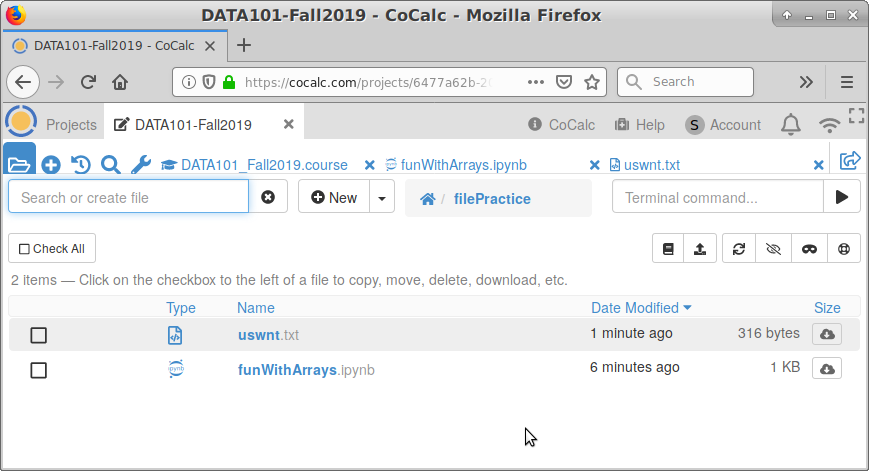
\includegraphics[width=0.9\textwidth]{folder.png}
\medskip
\caption{A directory (folder) on CoCalc, which contains two files: a plain-text
file (called \texttt{uswnt.txt}) and a Jupyter Notebook which will read from it
(\texttt{funWithArrays.ipynb}).}
\label{fig:folder}
\end{figure}

\index{extension@extension (filename)}
\index{filename extension}
\index{US Women's National Team}
\index{soccer}

The two entries listed are a plain-text file (called \texttt{uswnt.txt}) and a
Jupyter Notebook (\texttt{funWithArrays.ipynb}). You can tell that the former
is a plain-text file because of the \textbf{filename extension}
``\texttt{.txt}''. If we clicked on \texttt{uswnt.txt}, we'll bring up the
contents of the file, as shown in Figure~\ref{fig:textFile}. In this case, we
have the current roster on the US Women's National Soccer team, one name per
line. Perhaps the most important thing to see is that the file itself, which we
will read into Python in a moment, is nothing strange or scary: you could type
it yourself into Notepad or Word.\footnote{If you do ever create a plain-text
file using Microsoft Word or similar word processing program, be sure to choose
``Save as...'' and save the file in \textbf{plain-text mode}. If you don't,
Word will save a ton of extraneous formatting information (page settings,
fonts, italics, and so forth) which will utterly pollute the raw information
and make it impossible to read into Python.}

\index{camel case}

This is a good time to mention that \textit{spaces and other funny characters
in filenames are considered evil.} You might think it looks better to call the
notebook file ``\texttt{fun with arrays.ipynb}'' and the data file ``\texttt{US
Women's National Team roster.txt''}, but I promise you it will lead to pain in
the end, for a variety of fiddly reasons. It's better to use \textbf{camel
case} for filenames, which is simply
capitalizingEachSuccessive\-Word\-InAPhrase.

\begin{figure}[ht]
\centering
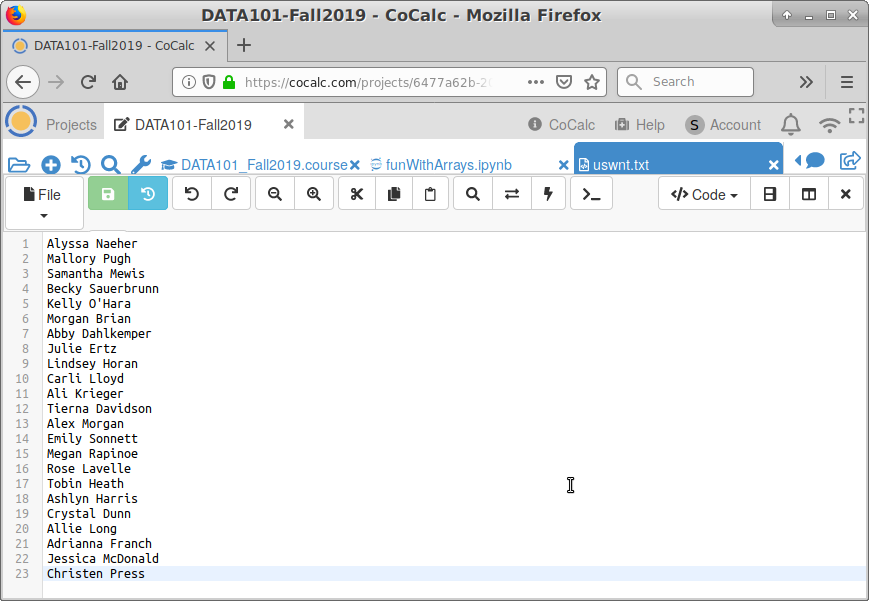
\includegraphics[width=0.8\textwidth]{textFile.png}
\medskip
\caption{The contents of a plain-text file, as rendered by CoCalc.}
\label{fig:textFile}
\end{figure}

Okay, finally back to NumPy code. If all the stars are aligned, we can write
this code in a \texttt{funWithArrays.ipynb} cell to read the soccer roster into
an \texttt{ndarray}:

\begin{Verbatim}[fontsize=\small,samepage=true,frame=single,framesep=3mm]
roster = np.loadtxt("uswnt.txt", dtype=object, delimiter="###")
\end{Verbatim}

\index{atomic}
\index{dtype@\texttt{.dtype}}
\index{object@\texttt{object} (for \texttt{loadtxt()})}
There's a lot of weird stuff in that line, so follow me here. The first
argument is easy enough: the name of the file that contains our data. (Again, I
stress that the file must be located \textit{in the same directory} as the
notebook!) The second argument is bizarre: we know what \texttt{dtype} means,
but ``\texttt{object}''? Ugh, another fiddly detail. When you read from a file
into a NumPy array, you will be reading one of our three atomic types. Here are
the rules:

\begin{center}
\begin{tabular}{c|c}
If you want to read an array of... & ...then set \texttt{dtype} to: \\
\hline
\texttt{int}s & \texttt{int} \\
\texttt{float}s & \texttt{float} \\
\texttt{str}s & \texttt{object} \\
\end{tabular}
\end{center}

So basically, you set \texttt{dtype} to the type of data you want in your
\texttt{ndarray}...unless you want strings, in which case you put the word
\texttt{object}. Sorry about that.

\index{delimiter}

The last of the three arguments is even nuttier, and you actually don't need to
include it at \textit{all} if you're reading \texttt{int}s or \texttt{float}s.
If you're reading \texttt{str}s, however, you need to set the
\textbf{delimiter} to something \textit{that doesn't appear in any of the
\texttt{str}s}. I chose three-hashtags-in-a-row since that rarely appears in
any set of text data.

Bottom line: once we've done all this, we get:

\begin{Verbatim}[fontsize=\small,samepage=true,frame=single,framesep=3mm]
print(roster)
\end{Verbatim}

\begin{Verbatim}[fontsize=\small,samepage=true,frame=leftline,framesep=5mm,framerule=1mm]
['Alyssa Naeher' 'Mallory Pugh' 'Samantha Mewis' 'Becky Sauerbrunn'
 "Kelly O'Hara" 'Morgan Brian' 'Abby Dahlkemper' 'Julie Ertz'
 'Lindsey Horan' 'Carli Lloyd' 'Ali Krieger' 'Tierna Davidson'
 'Alex Morgan' 'Emily Sonnett' 'Megan Rapinoe' 'Rose Lavelle'
 'Tobin Heath' 'Ashlyn Harris' 'Crystal Dunn' 'Allie Long'
 'Adrianna Franch' 'Jessica McDonald' 'Christen Press']
\end{Verbatim}

which is pretty cool.

\begin{figure}[ht]
\centering
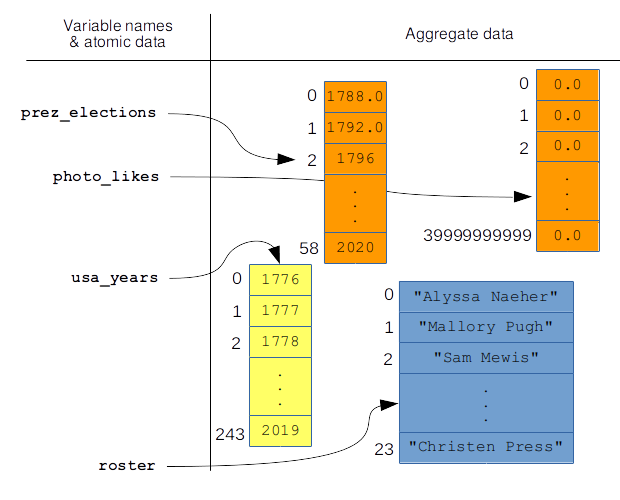
\includegraphics[width=1\textwidth]{arraysInMemory.png}
\caption{The memory picture of the four arrays we created in
section~\ref{sec:creatingArrays}.}
\label{fig:arraysInMemory}
\end{figure}
\section{Arrays in memory pictures}

\index{pointer}

Before we leave this chapter and move on to actually \textit{using} the
\texttt{ndarrays} we've created, let me once again emphasize the memory picture
and where arrays live in it. The four arrays we created in the previous section
are depicted in Figure~\ref{fig:arraysInMemory} on the following page. In each
case, the variable name appears in the left half, with a pointer to the array
itself which lives in the right half. All four arrays start at index 0, of
course, and is numbered up to its length minus 1.

Learn to love these pictures!
